% !TeX spellcheck = pt_BR

%%%%%%%%%%%%%%%%%%%%%%%%%%%%%%%%%%%%%%%%%%%%%%%
% Modelo adaptado do template original de
% Ted Pavlic (http://www.tedpavlic.com)
% Todos os créditos a ele.
%
% Na versão atual, o que foi modificado
% do original:
% Ajusta a numeração das questões e
% passa para português.
% Além de separar as configurações
% em um arquivo .cls separado.
%
% Crédito ao Roberto por ter feito
% a maior parte do trabalho de passar
% para o português e fazer outros
% ajustes para a versão atual deste template.
%%%%%%%%%%%%%%%%%%%%%%%%%%%%%%%%%%%%%%%%%%%%%%%


%----------------------------------------------------------------------------------------
%	PACKAGES E OUTRAS CONFIGURAÇÕES
%----------------------------------------------------------------------------------------

\documentclass{homeworkclass}

\usepackage{myMacros}


\hmwkTitle{Lista\ de\ Exercícios \#2}
\hmwkDueDate{Quinta,\ 28\ de\ Março,\ 2019}
\hmwkClass{CPE723 Otimização Natural}
\hmwkClassTime{Terças e Quintas: 08:00-10:00}
\hmwkClassInstructor{Prof. José Gabriel Rodríguez Carneiro Gomese}
\hmwkAuthorName{Vinicius Mesquita de Pinho}
\hmwkAuthorShortName{Vinicius Mesquita}

\begin{document}

\maketitle

%----------------------------------------------------------------------------------------
%	SUMÁRIO
%----------------------------------------------------------------------------------------

%\setcounter{tocdepth}{1} % Uncomment this line if you don't want subsections listed in the ToC

\clearpage
\newpage
%\tableofcontents
%\newpage

%----------------------------------------------------------------------------------------
%	QUESTÃO 1
%----------------------------------------------------------------------------------------

% To have just one problem per page, simply put a \clearpage after each problem


\begin{homeworkProblem}

Considere um processo de Markov $X(t)$ que tem três estados possíveis: 0, 1 e 2. A evolução temporal deste processo é dada pela matriz de transição a seguir:
\begin{equation*}
M = \begin{bmatrix}
0.5 & 0.25 & 0.25 \\
0.25 & 0.50 & 0.25 \\
0.25 & 0.25 & 0.50
\end{bmatrix}
\end{equation*}
\begin{homeworkSection}[a) Considerando que a distribuição de probabilidade de $X(0)$ é dada pelo vetor $\pbf_{0} = \left( 0.3 \, \, 0.4 \, \, 0.3 \right)^{\Trm}$, calcule a distribuição de probabilidade de $X(3)$ (ou seja, do processo de Markov no instante $t = 3$).]

A distribuição de probabilidade de $X(1)$ pode ser calculada a partir da cadeia de Markov da seguinte maneira:
\begin{equation*}
	\pbf_{1} = \Mbf \pbf_{0}.
\end{equation*}
A distribuição de probabilidade de $X(2)$, seguindo a mesma ideia:
\begin{equation*}
	\pbf_{2} = \Mbf^{2} \pbf_{1}.
\end{equation*}
Logo, a distribuição de probabilidade de $X(3)$, pode ser obtida por:
\begin{equation*}
	\pbf_{3} = \Mbf^{3} \pbf_{2}.
\end{equation*}
Usando os valores dados pela questão, obtemos o seguinte vetor $\pbf_{3}^{\Trm} = \left( 0.3593 \, \, 0.3489 \, \, 0.3463 \right)$.
\end{homeworkSection}


\begin{homeworkSection}[b)Iniciando em $X(0) = 1$, e usando um gerador de números aleatórios (são necessários apenas três números aleatórios equiprováveis), calcule manualmente uma amostra do processo X(t) até $t = 3$.]

O código usado para a questão.
\begin{lstlisting}[language=Python]
	M = np.matrix('0.50 0.25 0.25; 0.25 0.50 0.25; 0.25 0.25 0.50')
	estado_atual = 1
	tempos_possiveis = np.array([1, 2, 3])
	soma_coluna = 0
	iterador = 0

	for t in tempos_possiveis:
		uniforme_sorteado = np.random.uniform(0,1)
		while uniforme_sorteado > soma_coluna:
			soma_coluna = soma_coluna + M[estado_atual,iterador]
			iterador += 1
		print(f'no tempo {t} => mudança de estado: de {estado_atual} para
		... {iterador}. uniforme sorteado foi {uniforme_sorteado:.3}')
		estado_atual = iterador
\end{lstlisting}

As saídas encontradas: \\
No tempo 1 => Mudança de estado: de 1 para 2. Uniforme sorteado foi 0.441. \\
No tempo 2 => Mudança de estado: de 2 para 2. Uniforme sorteado foi 0.564. \\
No tempo 3 => Mudança de estado: de 2 para 3. Uniforme sorteado foi 0.773.
\end{homeworkSection}


\begin{homeworkSection}[c) Usando um computador, execute 100 repetições do item (b). Em cada uma das 100 repetições, comece a simulação com um valor diferente de $X(0)$, assumindo que os eventos $X(0) = 0$, $X(0) = 1$ e $X(0) = 2$ são equiprováveis. Armazene as 100 cadeiras obtidas em uma matriz $\Xbf$, com 4 colunas ($t = 0$ até $t = 3$) e 100 linhas.]

\begin{lstlisting}[language=Python]
	numero_iteracoes = 100
	escolhas = np.random.choice(3, numero_iteracoes)
	M = np.matrix('0.50 0.25 0.25; 0.25 0.50 0.25; 0.25 0.25 0.50')
	tempos_possiveis = np.array([0, 1, 2, 3])
	X = np.zeros((numero_iteracoes,4))

	for iteracoes in range(0,numero_iteracoes):
		soma_coluna = 0
		iterador = 0
		estado_inicial = escolhas[iteracoes]
		estado_atual = estado_inicial

		for t in tempos_possiveis:
			X[iteracoes,t] = estado_atual
			uniforme_sorteado = np.random.uniform(0,1)
			while uniforme_sorteado > soma_coluna:
				soma_coluna = soma_coluna + M[estado_atual,iterador]
				iterador += 1
			estado_atual = iterador
\end{lstlisting}


\end{homeworkSection}




\begin{homeworkSection}[d) Fazendo histogramas de cada uma das 4 colunas, calcule as distribuições de probabilidade do processo $X(t)$ em cada um dos 4 instantes: $t = 0, \, 1 \, 2 \, 3$. Comente os resultados obtidos.]

Podemos ver que para $100$ iterações, as probablidades ainda não ficam concentradas em apenas um estado, mas é possível que seja essa situação em mais iterações.

	\begin{figure}[!h]
		\centering
		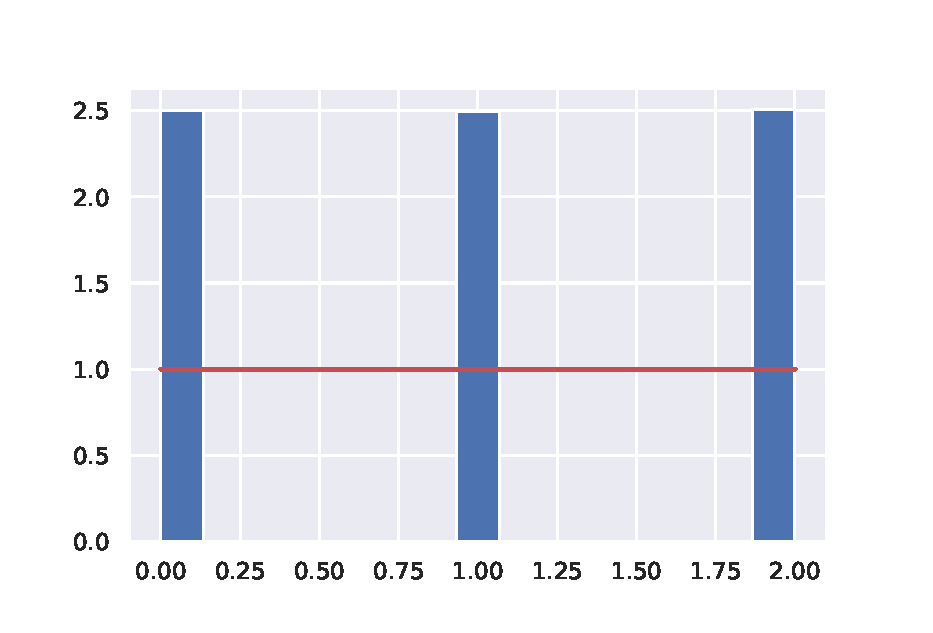
\includegraphics[width=0.7\linewidth]{figs/t_zero}
		\caption{t = 0}
	\end{figure}

	\begin{figure}[!h]
		\centering
		\includegraphics[width=0.7\linewidth]{figs/t_um}
		\caption{t = 1}
	\end{figure}

	\begin{figure}[!h]
		\centering
		\includegraphics[width=0.7\linewidth]{figs/t_dois}
		\caption{t = 2}
	\end{figure}

	\begin{figure}[!h]
		\centering
		\includegraphics[width=0.7\linewidth]{figs/t_tres}
		\caption{t = 3}
	\end{figure}


\end{homeworkSection}




\end{homeworkProblem}
\clearpage
%----------------------------------------------------------------------------------------
%	QUESTÃO 2
%----------------------------------------------------------------------------------------

\begin{homeworkProblem}
Considere um sistema em que só há 5 estados possíveis: $x = 1$, $x = 2$, $x = 3$, $x = 4$ e $x = 5$. Os custos de $J(x)$ De cada um dos estados são indicados na tabela abaixo:

\begin{center}
	\begin{tabular}{|c|c|}
		\hline
		$x$ & $J(x)$ \\
		\hline
		1 & 0.5 \\
		\hline
		2 & 0.2 \\
		\hline
		3 & 0.3 \\
		\hline
		4 & 0.1 \\
		\hline
		5 & 0.5 \\
		\hline
	\end{tabular}
\end{center}

\begin{homeworkSection}[a) Considere um processo de Markov gerado pela aplicação do algoritmo de Metropolis aos dados da tabela acima, com temperatura fixa $T = 0.1$. Calcule a matriz de transição $M$ que define o processo de $X(t)$. Obs: note que o estado $X(t)$ é unidimensional, e portanto a matriz $M$ é $5 \times 5$.]

Para este exercício, o seguinte código de Python foi utilizado:

\begin{lstlisting}[language=Python]
# estados possíveis
estados_possiveis = np.array([1, 2, 3, 4, 5])
energias_possiveis = np.array([0.5, 0.2, 0.3, 0.1, 0.4])
temperatura = 0.1

#A matriz de transição M, que será 5x5
M = np.zeros((5,5))
qtd_est_possi = len(estados_possiveis)

for ite_ou in range(0,qtd_est_possi):
	for ite_in in range(0,qtd_est_possi):
		delta_J = energias_possiveis[ite_ou] - energias_possiveis[ite_in]

		if (delta_J > 0):
			M[ite_in,ite_ou] = 1/qtd_est_possi
		else:
			if ite_in == ite_ou:
				M[ite_in,ite_ou] =  M[ite_ou,ite_ou]
				+ 1/(qtd_est_possi)*(np.exp(delta_J/temperatura))
				M[ite_ou,ite_ou] =  M[ite_ou,ite_ou]
				+ 1/(qtd_est_possi)*((1 - np.exp(delta_J/temperatura)))
			else:
				M[ite_in,ite_ou] = 1/(qtd_est_possi)*(np.exp(delta_J/temperatura))
				M[ite_ou,ite_ou] =  M[ite_ou,ite_ou]
				+ 1/(qtd_est_possi)*((1 - np.exp(delta_J/temperatura)))
\end{lstlisting}

A matriz $M$ calculada:

\begin{equation*}
M = \begin{bmatrix}
0.2 & 0.00995741 & 0.02706706 & 0.00366313 & 0.07357589\\
0.2 & 0.68939964& 0.2       & 0.07357589 &0.2       \\
0.2 & 0.07357589& 0.49935706& 0.02706706 & 0.2       \\
0.2 & 0.2       & 0.2       & 0.88573651 & 0.2       \\
0.2 & 0.02706706& 0.07357589& 0.00995741 & 0.32642411
\end{bmatrix}
\end{equation*}

\end{homeworkSection}

\begin{homeworkSection}[b) Iniciando em $X(0) = 1$, calcule manualmente 4 amostras do processo X(t).]

\begin{lstlisting}[language=Python]
estado_atual = 1
tempos_possiveis = np.array([1, 2, 3, 4])
soma_coluna = 0

iterador = 0

for t in tempos_possiveis:
	uniforme_sorteado = np.random.uniform(0,1)
	while uniforme_sorteado > soma_coluna:
		soma_coluna = soma_coluna + M[estado_atual,iterador]
		iterador += 1
	print(f'No tempo {t} => Mudança de estado: de {estado_atual}
	 para {iterador}. Uniforme sorteado foi {uniforme_sorteado:.3}.')
	estado_atual = iterador
	\end{lstlisting}

	No tempo 1 => Mudança de estado: de 1 para 2. Uniforme sorteado foi 0.431. \\
	No tempo 2 => Mudança de estado: de 2 para 2. Uniforme sorteado foi 0.227. \\
	No tempo 3 => Mudança de estado: de 2 para 2. Uniforme sorteado foi 0.148. \\
	No tempo 4 => Mudança de estado: de 2 para 2. Uniforme sorteado foi 0.145.
\end{homeworkSection}

\begin{homeworkSection}[c) Qual é o vetor invariante da matriz $M$ do item (a)? Obs: para facilitar os cálculos, pode-se usar o computador neste item.]
\begin{lstlisting}[language=Python]
	autovalores,autovetores = np.linalg.eig(M)
	vetor_pi = autovetores[:,0]/np.sum(autovetores[:,0])
	vetor_pi
\end{lstlisting}
O vetor encontrrado foi $\pibf = \left( 0.011 \, \, 0.23 \, \, 0.08 \, \, 0.63 \, \, 0.03 \right)^{\Trm}$

\end{homeworkSection}

\begin{homeworkSection}[d) Calcule os fatores de Boltzmann (ou seja, $e^{-(J(x)/T)}$) associados aos dados da tabela acima, e compare-os com o resultado do item (c). Use $T = 0.1$.]

\begin{lstlisting}[language=Python]
	fatores_boltzmann = np.exp(-energias_possiveis/temperatura)
	outro_vetor_pi = fatores_boltzmann/np.sum(fatores_boltzmann)
	outro_vetor_pi
\end{lstlisting}
O vetor encontrrado foi $\pibf = \left( 0.011 \, \, 0.23 \, \, 0.08 \, \, 0.63 \, \, 0.03 \right)^{\Trm}$

\end{homeworkSection}

\begin{homeworkSection}[e) Simulated Annealing: Usando um computador, execute 1000 iterações do algoritmo de Metropolis em cada uma das 10 temperaturas a seguir. Na passagem de uma temperatura para a outra, use o estado atual. Comente as distribuições de probabilidade obtidas no final de cada temperatura.]

	\begin{lstlisting}[language=Python]
		temperaturas = np.array([0.1, 0.0631, 0.05, 0.0431, ...
		0.0387, 0.0356, 0.0333, 0.0315, 0.0301, 0.0289])
		qtd_temp = len(temperaturas)
		total_iteracoes = 1000
		estados_possiveis = np.array([0, 1, 2, 3, 4])
		qtd_est_possi = len(estados_possiveis)
		energias_possiveis = np.array([0.5, 0.2, 0.3, 0.1, 0.4])

		histogram_matrix = np.zeros((qtd_est_possi,qtd_temp))
		estado_inicial = np.random.choice(qtd_est_possi)
		estado_atual = estado_inicial
		J_inicial = energias_possiveis[estado_inicial]
		J_atual = J_inicial

		todos_J = np.zeros((total_iteracoes,qtd_temp))
		todos_estados = np.zeros((total_iteracoes,qtd_temp))

		for ite_out in range(0,qtd_temp):
			for ite_in in range(0,total_iteracoes):
				estado_possivel = np.random.choice(qtd_est_possi)
				J = energias_possiveis[estado_possivel]
				r = np.random.uniform(0,1)
				if (r <  np.exp((J_atual-J)/temperaturas[ite_out])):
					estado_atual = estado_possivel
					J_atual = J
				todos_estados[ite_in,ite_out] = estado_atual
				todos_J[ite_in,ite_out] = J_atual
			histogram_matrix[:,ite_out], binq, outroq =
			plt.hist(todos_estados[:,ite_out], qtd_est_possi, density=True)
			histogram_matrix[:,ite_out] = histogram_matrix[:,ite_out] /
			np.sum(histogram_matrix[:,ite_out] )
	\end{lstlisting}


\begin{equation*}
M = \begin{bmatrix}
0.009 & 0.159 & 0.111 & 0.051 & 0.046 & 0.039 & 0.057 & 0.012 & 0.057 &
0.022 \\
0.216 & 0.028 & 0.008 & 0.    & 0.    & 0.    & 0.    & 0.    & 0.    &
0.   \\
0.064 & 0.    & 0.    & 0.    & 0.001 & 0.    & 0.004 & 0.001 & 0.    &
0.002 \\
0.693 & 0.81  & 0.88  & 0.    & 0.    & 0.    & 0.    & 0.    & 0.    &
0.   \\
0.018 & 0.003 & 0.001 & 0.949 & 0.953 & 0.961 & 0.939 & 0.987 & 0.943 & 0.976
\end{bmatrix}
\end{equation*}
É possível ver que temos uma concentração da probabilidade em um terminado estado no final.

\end{homeworkSection}



\end{homeworkProblem}
%----------------------------------------------------------------------------------------
%	QUESTÃO 3
%----------------------------------------------------------------------------------------

\begin{homeworkProblem}
Proponha uma função $J(\xbf)$, sendo $\xbf$ um vetor com 10 dimensões, cujo ponto mínimo você conheça. Evite propor funções que tenham um só ponto mínimo. Encontre o ponto mínimo global utilizando S.A. Obs: Neste exercício, entregue o código utilizando e alguns comentários sobre o resultado obtido.
\end{homeworkProblem}

\begin{figure}[!h]
	\centering
	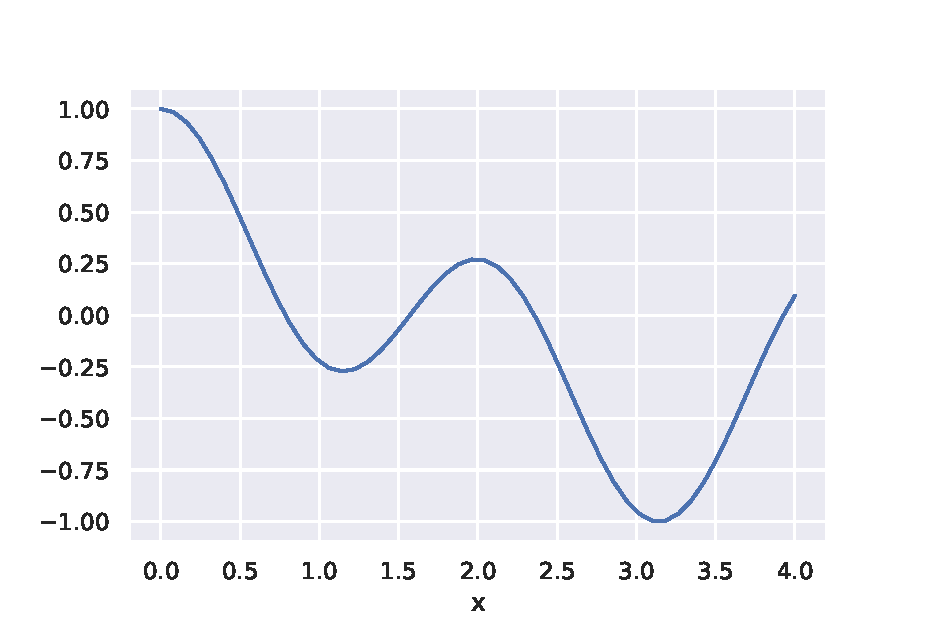
\includegraphics[width=0.7\linewidth]{figs/cos}
\end{figure}

\begin{lstlisting}[language=Python]
	J_inicial = chosen_function(pt_inicial)
	pt_atual = pt_inicial
	J_atual = J_inicial

	# Parametros utilizados
	N = 100
	K = 8
	T_inicial = 5e-1
	T = T_inicial
	epsilon = 10e-2

	fim = 0
	n = 0
	k = 1
	J_min = J_atual
	pt_min = pt_atual

	while not(fim):
		n = n + 1
		pt = pt_atual + epsilon*(np.random.normal(0, 1))
		J = chosen_function(pt)
		todos_J = np.append(todos_J,J)
		if (np.random.uniform(0,1) < np.exp((J_atual-J)/T)):
			pt_atual = pt
			J_atual = J
		if (J < J_min):
			J_min = J
			pt_min = pt
		if (n % N == 0):
			k = k + 1
			T = T_inicial/(np.log(1+k))
			if k == K:
				fim = 1
	pt_min
\end{lstlisting}


\end{document}